\documentclass{article}

% Language setting
% Replace `english' with e.g. `spanish' to change the document language
\usepackage[english]{babel}

% Set page size and margins
% Replace `letterpaper' with`a4paper' for UK/EU standard size
\usepackage[letterpaper,top=2cm,bottom=2cm,left=3cm,right=3cm,marginparwidth=1.75cm]{geometry}

% Useful packages
\usepackage{amsmath}
\usepackage{amssymb}
\usepackage{graphicx}
\usepackage{enumitem}
\usepackage[colorlinks=true, allcolors=blue]{hyperref}

\usepackage{hyperref}
\hypersetup{
    colorlinks=true,
    linkcolor=blue,
    filecolor=magenta,      
    urlcolor=cyan,
    pdftitle={Overleaf Example},
    pdfpagemode=FullScreen,
    }

\urlstyle{same}

\usepackage{tikz-cd}

%%%%%%%%%%% Box pacakges and definitions %%%%%%%%%%%%%%
\usepackage[most]{tcolorbox}
\usepackage{xcolor}

% Define the colors
\definecolor{boxheader}{RGB}{0, 51, 102}  % Dark blue
\definecolor{boxfill}{RGB}{173, 216, 230}  % Light blue

% Define the tcolorbox environment
\newtcolorbox{mathdefinitionbox}[2][]{%
    colback=boxfill,   % Background color
    colframe=boxheader, % Border color
    fonttitle=\bfseries, % Bold title
    coltitle=white,     % Title text color
    title={#2},         % Title text
    enhanced,           % Enable advanced features
    attach boxed title to top left={yshift=-\tcboxedtitleheight/2}, % Center title
    boxrule=0.5mm,      % Border width
    sharp corners,      % Sharp corners for the box
    #1                  % Additional options
}
%%%%%%%%%%%%%%%%%%%%%%%%%

\usepackage{biblatex}
\addbibresource{sample.bib}


%%%%%%%%%%% New Commands %%%%%%%%%%%%%%
\newcommand*{\T}{\mathcal T}
\newcommand*{\cl}{\text cl}


\newcommand{\ket}[1]{|#1 \rangle}
\newcommand{\bra}[1]{\langle #1|}
\newcommand{\inner}[2]{\langle #1 | #2 \rangle}
\newcommand{\R}{\mathbb{R}}
\newcommand{\C}{\mathbb{C}}
\newcommand{\V}{\mathbb{V}}
\newcommand{\Hilbert}{\mathcal{H}}
\newcommand{\oper}{\hat{\Omega}}
\newcommand{\lam}{\hat{\Lambda}}

\newcommand{\bigslant}[2]{{\raisebox{.2em}{$#1$}\left/\raisebox{-.2em}{$#2$}\right.}}
\newcommand{\restr}[2]{{% we make the whole thing an ordinary symbol
  \left.\kern-\nulldelimiterspace % automatically resize the bar with \right
  #1 % the function
  \vphantom{\big|} % pretend it's a little taller at normal size
  \right|_{#2} % this is the delimiter
  }}
%%%%%%%%%%%%%%%%%%%%%%%%%%%%%%%%%%%%%%%


\newtcolorbox{dottedbox}[1][]{%
    colback=white,    % Background color
    colframe=white,    % Border color (to be overridden by dashrule)
    sharp corners,     % Sharp corners for the box
    boxrule=0pt,       % No actual border, as it will be drawn with dashrule
    boxsep=5pt,        % Padding inside the box
    enhanced,          % Enable advanced features
    overlay={\draw[dashed, thin, black, dash pattern=on \pgflinewidth off \pgflinewidth, line cap=rect] (frame.south west) rectangle (frame.north east);}, % Dotted line
    #1                 % Additional options
}

\tcbset{theostyle/.style={
    enhanced,
    sharp corners,
    attach boxed title to top left={
      xshift=-1mm,
      yshift=-4mm,
      yshifttext=-1mm
    },
    top=1.5ex,
    colback=white,
    colframe=blue!75!black,
    fonttitle=\bfseries,
    boxed title style={
      sharp corners,
    size=small,
    colback=blue!75!black,
    colframe=blue!75!black,
  } 
}}

\newtcbtheorem[number within=section]{Theorem}{Theorem}{%
  theostyle
}{thm}

\newtcbtheorem[number within=section]{Definition}{Definition}{%
  theostyle
}{def}



\title{Math H185 Homework 1}
\author{Keshav Balwant Deoskar}

\begin{document}
\maketitle

% \vskip 0.5cm
% \pagebreak 

%%%%%%%%%%%%%%%%%%%%%%%%%%%%%%%%%%%%%%%%%%%%%%%%%%%%%%%%%%%%%%%%%
\begin{mathdefinitionbox}{Question 1}
\vskip 0.5cm
  \begin{enumerate}[label=(\alph*)]
    \item Prove that if $z \in \mathbb{C}$ then $z \bar{z} = |z|^2$.
    \item Prove that if $z, w \in \mathbb{C}$ then $\overline{z \cdot w} = \bar{z} \cdot \bar{w}$.
    \item Use parts (a) and (b) to show that for complex numbers $w, z \in \mathbb{C}$, 
    \[ |z \cdot w| = |z| \cdot |w| \]
  \end{enumerate}
\end{mathdefinitionbox}
%%%%%%%%%%%%%%%%%%%%%%%%%%%%%%%%%%%%%%%%%%%%%%%%%%%%%%%%%%%%%%%%%

\vskip 0.5cm
\underline{\textbf{Proof:}} 
\begin{enumerate}[label=(\alph*)]
  \item Consider $z = a + bi \in \C$. Then, $\bar{z} = a - bi$, and 
  \begin{align*}
    z \cdot \bar{z} &= (a + bi) \cdot (a - bi) \\
    &= a \cdot a - a \cdot bi + bi \cdot a + (bi) \cdot (-bi) \\
    &= a^2 - b^2 \cdot (-1) \\
    &= a^2 + b^2 \\
    &= |z|^2
  \end{align*}
  So, 
  \[ \boxed{z \cdot \bar{z} = |z|^2} \]
  \vskip 0.5cm

  \item Now, suppose we have $z = a + bi$ and $w = c + di$. Then, 
  \begin{align*}
    z \cdot w &= (a + bi) \cdot (c + di) \\
    &= (ac - bd) + (ad + bc)i
  \end{align*}
  So, 
  \begin{equation}
    \overline{z \cdot w} = (ac - bd) - (ad + bc)i
  \end{equation}

  Now,
  \begin{align}
    \overline{z} \cdot \overline{w} &= (a - bi) \cdot (c - di) \\
    &= (ac - bd) - (bc + ad)i
  \end{align}

  So, from equations (1) and (3), we see that 
  \[ \boxed{\overline{z \cdot w} = \overline{z} \cdot \overline{w}} \]

  \vskip 0.5cm
  \item Now,  
  \[ |z \cdot w|^2 = (z \cdot w) \cdot (\overline{z \cdot w}) = z \cdot w \cdot \overline{z} \cdot \overline{w} \]
  
  (first equality due to part (a) and second due to part (b)).
  \vskip 0.5cm

  Using commutativity and associativity of complex multiplication, we can write 
  \begin{align*}
    (z \cdot w) (\overline{z \cdot w}) &= (z \cdot w) (\overline{w} \cdot \overline{z}) \\
    &= z \cdot (w \cdot \overline{w}) \cdot \overline{z} \\
    &= z \cdot \overline{z} \cdot  (w \cdot \overline{w}) \\
    &= |z|^2 \cdot  |w|^2 
  \end{align*}
  And since the norm of a complex number is guaranteed to be positive (or zero), we can take the square root on both sides without uncertainty and conclude that 
  \[ \boxed{|z \cdot w| = |z| \cdot |w|} \]
\end{enumerate}

\vskip 0.5cm
\hrule 
\vskip 0.5cm


%%%%%%%%%%%%%%%%%%%%%%%%%%%%%%%%%%%%%%%%%%%%%%%%%%%%%%%%%%%%%%%%%
\begin{mathdefinitionbox}{Question 2}
\vskip 0.5cm
  Draw a picture of the following subsets of $\C$.
  \begin{enumerate}[label=(\alph*)]
    \item $\{ z \in \C : |z - 6i| \leq 1 \}$
    \item $\{ z \in \C : \text{Im}(z) = \text{Re}(z)^2 \}$
    \item $\{ z \in \C : |z| = \text{Re}(z) + 1 \}$
  \end{enumerate}
\end{mathdefinitionbox}
%%%%%%%%%%%%%%%%%%%%%%%%%%%%%%%%%%%%%%%%%%%%%%%%%%%%%%%%%%%%%%%%%

\vskip 0.5cm
\underline{\textbf{Answer:}} 

\begin{enumerate}[label=(\alph*)]
  \item This is the disk of radius $1$ centered at the point $6i$.

  \vskip 0.5cm
  \item This is a parabola.
  
  \vskip 0.5cm
  \item Consider $z = a + bi \in \C$. We know that $|z| = \sqrt{a^2 + b^2}$, so this region is 
  \begin{align*}
    &a^2 + b^2 = (a + 1)^2\\
    \implies &a^2 + b^2 = a^2 + 2a + 1 \\
    \implies &b^2 = 2a + 1 \\
    \implies &a = \frac{b^2 - 1}{2}
  \end{align*}
  That is, the set is a horizontal parabola opening up to the right, with vertex at $z = i$.

\end{enumerate}

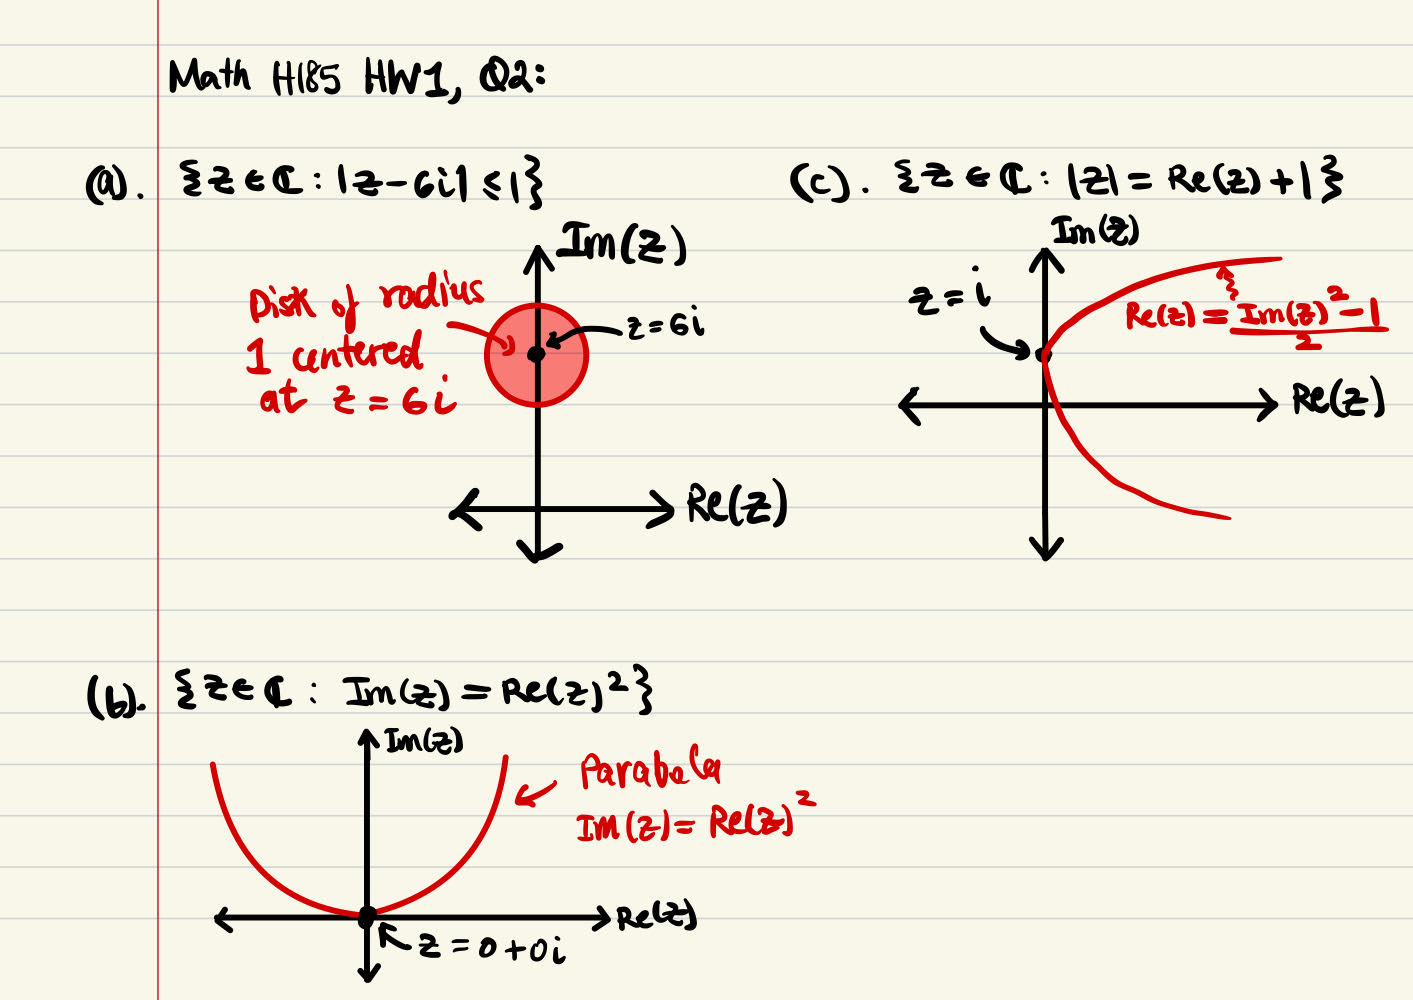
\includegraphics[scale=0.30]{Q2.jpg}

\vskip 0.5cm
\hrule 
\vskip 0.5cm


%%%%%%%%%%%%%%%%%%%%%%%%%%%%%%%%%%%%%%%%%%%%%%%%%%%%%%%%%%%%%%%%%
\begin{mathdefinitionbox}{Question 3}
  \vskip 0.5cm
  Express the following complex numbers in the form $a + bi$ where $a, b \in \R$.
    \begin{enumerate}[label=(\alph*)]
      \item $(12 + 15i) + (-5 - 8i)$ 
      \item $(4 + 7i) (5 - 2i)$ 
      \item $\frac{3}{i}$ 
      \item $\frac{169}{5 + 12i}$ 
    \end{enumerate}
  \end{mathdefinitionbox}
  %%%%%%%%%%%%%%%%%%%%%%%%%%%%%%%%%%%%%%%%%%%%%%%%%%%%%%%%%%%%%%%%%
  
  \vskip 0.5cm
  \underline{\textbf{Answer:}} 
  
  \begin{enumerate}[label=(\alph*)]
    \item \begin{align*}
      (12 + 15i) + (-5 - 8i) &= (12 - 5) + (15 - 8)i \\
      &= 7 + 7i
    \end{align*}

    
    \item \begin{align*}
      (4 + 7i) (5 - 2i) &= 4(5) + 4(-2i) + (7i)(5) +(7i)(-2i) \\
      &= 20 - 8i + 35i + 14 \\
      &= 34 + 17i
    \end{align*} 

  
    \item \begin{align*}
      \frac{3}{i} &= \frac{3}{i} \cdot \frac{i}{i} \\
      &= \frac{3i}{-1} \\
      &= 0 - 3i
    \end{align*} 


    \item \begin{align*}
      \frac{169}{5 + 12i} &= \frac{169}{5 + 12i} \cdot \frac{5 - 12i}{5 - 12i}\\
      &= \frac{169 \cdot (5 - 12i)}{25 + 144} \\
      &= \frac{169}{169} \cdot (5 - 12i) \\
      &= 5 - 12i
    \end{align*} 
  \end{enumerate}
  
  \vskip 0.5cm
  \hrule 
  \vskip 0.5cm

%%%%%%%%%%%%%%%%%%%%%%%%%%%%%%%%%%%%%%%%%%%%%%%%%%%%%%%%%%%%%%%%%
\begin{mathdefinitionbox}{Question 4}
  \vskip 0.5cm
  Express the following complex numbers in the form $a + bi$ where $a, b \in \R$.
    \begin{enumerate}[label=(\alph*)]
      \item $4 e^{\pi i / 4}$ 
      \item $2 e^{\pi i / 2} + 4 e^{4 \pi i / 3}$ 
      \item $(6 e^{\pi i / 6}) \cdot (6 e^{\pi i / 4})$ 
    \end{enumerate}
\end{mathdefinitionbox}
%%%%%%%%%%%%%%%%%%%%%%%%%%%%%%%%%%%%%%%%%%%%%%%%%%%%%%%%%%%%%%%%%
  
  \vskip 0.5cm
  \underline{\textbf{Answer:}} 

  \begin{enumerate}[label=(\alph*)]
    \item \underline{For $4 e^{\pi i / 4}$, we have:}
    \begin{align*}
      4 e^{\pi i / 4} &= 4 \cdot \left( \cos\left( \frac{\pi}{4} \right) + i\sin\left( \frac{\pi}{4} \right) \ \right) \\
      &= 4 \cdot \left( \frac{1}{\sqrt{2}} + i\frac{1}{\sqrt{2}} \right) 
    \end{align*}
    \[ \boxed{\implies 4 e^{\pi i / 4} = 2\sqrt{2} + 2\sqrt{2} \cdot i} \]
    
    \vskip 0.5cm
    \item \underline{For $2 e^{\pi i / 2} + 4 e^{4 \pi i / 3}$, we have:}
    \begin{align*}
      2 e^{\pi i / 2} + 4 e^{4 \pi i / 3} &= 2 \cdot \left( \cos\left( \frac{\pi}{2} \right) + i\sin\left( \frac{\pi}{2} \right) \right) + 4 \cdot \left( \cos\left( \frac{4\pi}{3} \right) + i\sin\left( \frac{4\pi}{3} \right) \right) \\ 
      &= 2 \cdot \left( \cos\left( \frac{\pi}{2} \right) + i\sin\left( \frac{\pi}{2} \right) \right) + 4 \cdot \left( \cos\left( \pi + \frac{\pi}{3} \right) + i\sin\left( \pi + \frac{\pi}{3} \right) \right) \\ 
      &= 2 \cdot \left( 0 + i \cdot 1 \right) + 4 \cdot \left( -\frac{1}{2} - i\frac{\sqrt{3}}{2} \right) \\
      &= (2 - 2) - 2\sqrt{3} i 
    \end{align*}
    \[ \boxed{\implies 2 e^{\pi i / 2} + 4 e^{4 \pi i / 3} = 0 - 2\sqrt{3} i} \]


    \vskip 0.5cm
    \item \underline{For $(6 e^{\pi i / 6}) \cdot (6 e^{\pi i / 4})$, we have:}
    \begin{align*}
      (6 e^{\pi i / 6}) \cdot (6 e^{\pi i / 4}) &= 36e^{\pi i \cdot \left(\frac{1}{6} + \frac{1}{4}\right)} \\
      &= 36e^{\pi i \cdot \left(\frac{4}{24} + \frac{6}{24}\right)} \\
      &= 36e^{\pi i \cdot \frac{10}{24}} \\
      &= 36 \cdot \left[ \cos\left( \frac{5\pi}{12} \right) + i \sin\left(\frac{5\pi}{12}  \right)\right] 
    \end{align*}
    \[ \boxed{\implies (6 e^{\pi i / 6}) \cdot (6 e^{\pi i / 4}) = 9.317485624 + 34.77332975i} \]

  \end{enumerate}

  \vskip 0.5cm
  \hrule 
  \vskip 0.5cm


%%%%%%%%%%%%%%%%%%%%%%%%%%%%%%%%%%%%%%%%%%%%%%%%%%%%%%%%%%%%%%%%%
\begin{mathdefinitionbox}{Question 5}
\vskip 0.5cm
Express the following complex numbers in the form $re^{i\theta}$ where $r \in \mathbb{R}_{\geq 0}$ and $\theta \in [0, 2\pi]$
  \begin{enumerate}[label=(\alph*)]
    \item $1 + \sqrt{3} i$ 
    \item $\sqrt{3} - i$ 
    \item $1 + i$ 
    \item $\frac{1}{1-i}$
  \end{enumerate}
\end{mathdefinitionbox}
%%%%%%%%%%%%%%%%%%%%%%%%%%%%%%%%%%%%%%%%%%%%%%%%%%%%%%%%%%%%%%%%%
  
\vskip 0.5cm
\underline{\textbf{Answer:}} 

\begin{enumerate}[label=(\alph*)]
  \item \underline{For $1 + \sqrt{3}$, we have:}
  \begin{align*}
    r &= \sqrt{1^2 + (\sqrt{3})^2} \\
    &= \sqrt{4} \\
    &= 2
  \end{align*}
  and 
  \begin{align*}
    \theta &= \arctan\left( \frac{\sqrt{3}}{1} \right) = \frac{\pi}{3}
  \end{align*}
  Thus, 
  \[ \boxed{ 1 + \sqrt{3} = 2 e^{\frac{1}{3} \pi i}} \]
  
  \vskip 0.5cm
  \item \underline{For $\sqrt{3} - i$, we have:}
  \begin{align*}
    r &= \sqrt{(\sqrt{3})^2 + (-i)^2} \\
    &= \sqrt{\left(\sqrt{3}\right)^2 + (-1)^2\cdot(i)^2} \\
    &= \sqrt{3 - 1} \\
    &= \sqrt{2}
  \end{align*}
  and
  \begin{align*}
    \theta &= \arctan\left( \frac{-1}{3} \right) \approx -0.32175055
  \end{align*}
  So, 
  \[ \boxed{\sqrt{3} - i = \sqrt{2}e^{-0.32175055 i}} \]


  \vskip 0.5cm
  \item \underline{For $1 + i$, we have:}
  \begin{align*}
    r = \sqrt{1^2 + 1^2} = \sqrt{2}
  \end{align*}
  and
  \begin{align*}
    \theta &= \arctan(1/1) = \frac{\pi}{4}
  \end{align*}
  \[ \boxed{1 + i = e^{\frac{\pi i }{4}}} \]

  \vskip 0.5cm
  \item \underline{For $\frac{1}{1-i} = \frac{1+i}{2}$, we have:}
  \begin{align*}
    r &= \sqrt{\left(\frac{1}{2}\right)^2 + \left(\frac{1}{2}\right)^2} \\
    &= \sqrt{2 \cdot \frac{1}{4}} \\
    &= \frac{1}{\sqrt{2}}
  \end{align*}
  and
  \begin{align*}
    \theta &= \arctan((1/2)/(-1/2)) \\
    &= \arctan(-1) \\
    &= 2\pi-\frac{\pi}{4} \\
    &= \frac{7\pi}{4}
  \end{align*}
  \[ \boxed{1 + i = \frac{1}{\sqrt{2}} e^{\frac{7\pi i }{4}}} \]
\end{enumerate}

\vskip 0.5cm
\hrule 
\vskip 0.5cm

%%%%%%%%%%%%%%%%%%%%%%%%%%%%%%%%%%%%%%%%%%%%%%%%%%%%%%%%%%%%%%%%%
\begin{mathdefinitionbox}{Question 6}
\vskip 0.5cm
Let $w = re^{i\theta}$ with $r > 0$, and $n > 0$ be a positive integer. Write down in terms of $r$, $\theta$, and $n$ the polar form of all complex numbers $z$ such that $z^{n} = w$.
\end{mathdefinitionbox}
%%%%%%%%%%%%%%%%%%%%%%%%%%%%%%%%%%%%%%%%%%%%%%%%%%%%%%%%%%%%%%%%%
  
\vskip 0.5cm
\underline{\textbf{Answer:}} 

In terms of the cartesian form $a + bi$, two complex numbers are the same if they have equal Real and Imaginary parts. In terms of polar coordinates, this means that they must have 
\begin{itemize}
  \item the same modulus, since $|z|^2 = \sqrt{a^2 + b^2}$ and the two equal complex numbers must both have $\text{Re}(z) = a, \text{Re}(z) = b$.
  \item their arguments, $\Theta_1, \Theta_2$ must be related as 
  \[ \Theta_1 - \Theta_2 = 2\pi \cdot k \]
  for some $k \in \mathbb{Z}$ because rotating around the origin by any integer multiple of $2\pi$ brings us back to the same point.
\end{itemize} 

\vskip 0.5cm
Let's denote $z$ in polar form as $z = Le^{i\tau}$. Then, in order to have $z^n = w$ we need 
\begin{align*}
  (Le^{i\tau})^n &= re^{i\theta} \\
  \implies L^ne^{i\cdot n\tau} &= re^{i\theta} \\
  \implies \frac{L^n}{r} e^{i \cdot \left( n\tau - \theta \right)} &= 1 \\
\end{align*}

Now, $|z \cdot w| = |z| \cdot |w|$, so 
\begin{align*}
  |1| &= \lvert \frac{L^n}{r} e^{i \cdot \left( n\tau - \theta \right)} \rvert \\
  \implies 1 &= \lvert \frac{L^n}{r} \rvert \cdot \lvert e^{i(n\tau - \theta)} \rvert \\
  \implies 1 &= \frac{|L^n|}{|r|}  \cdot \lvert e^{i(n\tau - \theta)} \rvert 
\end{align*}

But $|e^{iz}| = 1$ for any $z \in \C$. Thus, $\frac{|L^n|}{|r|} = \frac{|L|^n}{|r|} 1$ and since $L, r \in \R$ this simply means 
\[ \boxed{L = r^{1/n}} \]

\vskip 1cm
As for the argument, we know that $ \frac{L}{r} e^{i \cdot \left( n\tau - \theta \right)} = 1 + 0i$. That is, 
\[ \underbrace{(n\tau - \theta)}_{\Theta_1} - \underbrace{0}_{\Theta_2} = 2\pi k \] 
for $k \in \mathbb{Z}$.

\vskip 0.5cm
So, we have 
\[ \boxed{\tau = \frac{\left(2\pi k + \theta\right)}{n} } \]

\vskip 0.5cm
However, notice that we have some redundancy again. Both $k$ and $n$ are integers (and $n > 0$), so the values $k$ and $k' = k + m \cdot n$ where $m$ is any integer give the same value of $\tau$. So, really, the set of values for $k$ which give us \textbf{distinct} $\tau$ values is the Integers modulo $n$.


\vskip 0.5cm
Thus, in terms of $r, \theta, n$ the complex number $z$ must be of the form 
\[ \boxed{z = r^{1/n} e^{i \cdot \left(2\pi k + \theta\right)/n}} \]

where $k \in \mathbb{Z}/n\mathbb{Z}$, in order for the equation $z^n = w$ to hold.

\vskip 0.5cm
\hrule 
\vskip 0.5cm

%%%%%%%%%%%%%%%%%%%%%%%%%%%%%%%%%%%%%%%%%%%%%%%%%%%%%%%%%%%%%%%%%
\begin{mathdefinitionbox}{Question 7}
\vskip 0.5cm
Let $\{z_n = x_n + i y_n\}_n$ be a sequence of complex numbers. Prove that $\{z_n\}_n$ converges to $z \equiv x + iy$ if and only if $\lim_{x \rightarrow \infty} x_n = x$ and $\lim_{y \rightarrow \infty} y_n = y$. Here, $x_n, y_n, x, y \in \R$.
\end{mathdefinitionbox}
%%%%%%%%%%%%%%%%%%%%%%%%%%%%%%%%%%%%%%%%%%%%%%%%%%%%%%%%%%%%%%%%%
  
\vskip 0.5cm
\underline{\textbf{Answer:}} 
\vskip 0.5cm

\begin{itemize}
  \item \underline{$\implies$ Direction:} Suppose the sequence $\{z_n = x_n + iy_n\}$ converges to $z = x + iy$. Then, for any $\epsilon > 0$ there exists $N \in \mathbb{N}$ such that for all $n \geq N$, 
  \[ |z_n - z| < \epsilon \]
  \begin{align*}
    \implies& |(x_n + i y_n) - (x + iy)| < \epsilon \\
    \implies& |(x_n - x) + i(y_n - y)| < \epsilon \\
  \end{align*}
  
  Now, we know for all $z \in \C$ that $|\text{Re}(z)| < |z|$ and $|\text{Im}(z)| < |z|$.
  
  \begin{dottedbox}
    For $z = x + iy$, 
    \begin{align*}
      &x^2 < |z|^2 = x^2 + y^2 \;\; \text{ since $x^2, y^2 > 0$} \\
      \implies&x^2 < |z|
    \end{align*}
    and similarly for $y < |z|$
  \end{dottedbox}

  \vskip 0.5cm
  Therefore, 
  
  \begin{align*}
    &|x_n - x| < |(x_n - x) + i(y_n - y)| < \epsilon \\
    &|y_n - y| < |(x_n - x) + i(y_n - y)| < \epsilon 
  \end{align*}
  
  Therefore, the sequences $\{x_n\}$ and $\{y_n\}$ also converge.

  \vskip 0.5cm
  \item \underline{$\impliedby$ Direction:} Suppose the sequences $\{x_n\}$ and $\{y_n\}$ converge to $x$ and $y$ respectively. Then for any $\epsilon > 0$ there exist integers $N, M \geq 0$ such that for all $n \geq N$, $|x_n - x| < \epsilon$ and for all $m \geq M$, $|y_n - y| < \epsilon$.
  
  \vskip 0.5cm
  Find the values of $N, M$ corresponding to $\frac{\epsilon}{2} > 0$ and set $L = \max\{N, M\}$. Then, for all $l \geq L$ we have $|x_n - x| < \epsilon$ and $|y_n - y| < \epsilon$.

  \vskip 0.5cm
  Now, note that $|i (y_n - y)| = |i| \cdot |y_n - y| = |y_n - y|$. Using the Triangle Inequality, we have 
  \begin{align*}
    &|(x_n - x) + i(y_n - y)| \leq |x_n - x| + \underbrace{|i(y_n - y)|}_{=|y_n - y|} < \frac{\epsilon}{2} + \frac{\epsilon}{2} \\
    \implies& |(x_n + iy_n) - (x + iy) | < \epsilon
  \end{align*}
  Thus, 
  \[ \boxed{|z_n - z| < \epsilon} \]
  So, the sequence $\{z_n\}$ converges to $z$.
\end{itemize}

\vskip 0.5cm
\hrule 
\vskip 0.5cm

%%%%%%%%%%%%%%%%%%%%%%%%%%%%%%%%%%%%%%%%%%%%%%%%%%%%%%%%%%%%%%%%%
\begin{mathdefinitionbox}{Question 8}
\vskip 0.5cm
Let $f(z) = |z|$ be viewed as a function $f : \C \rightarrow \C$. Show that $f$ is not holomorphic at any $z \in \C$.
\end{mathdefinitionbox}
%%%%%%%%%%%%%%%%%%%%%%%%%%%%%%%%%%%%%%%%%%%%%%%%%%%%%%%%%%%%%%%%%
  
\vskip 0.5cm
\underline{\textbf{Answer:}} 

\vskip 0.5cm
For complex number $z = a + bi$, consider the function $f(z) = |z| = \sqrt{a^2 + b^2}$. The difference quotient is 

\begin{align*}
  \frac{f(z + h) - f(z)}{h} &= \frac{|z+h| - |z|}{h} \\
\end{align*}

Notice that the numerator is always a real number, whereas $h$ in the denominator may have an imaginary part. 
bh1
\vskip 0.5cm
Thus, for any $z \in \C$, if we approach the point $z$ horizontally i.e. $Im(h) = 0$ throughout the approach, then the difference quotient is a real number. However if we approach $z$ vertcally i.e. $Re(z) = 0$ throughout the approach, then the difference quotient is an imaginary number. Therefore, the function is not holomorphic anywhere.

\vskip 0.5cm
\hrule 
\vskip 0.5cm

% \printbibliography

\end{document}
